\documentclass[a4paper, 11pt]{article}

\usepackage{fullpage}

\usepackage[english,russian]{babel}
\usepackage[utf8]{inputenc}
\usepackage{amsmath, amsfonts, amssymb, amsthm}
\usepackage{mathtools}
\usepackage{bm}

\usepackage{hyperref}
\usepackage{booktabs}
\usepackage{graphicx}
\usepackage{subcaption}

\usepackage[linesnumbered,ruled,vlined]{algorithm2e}
\SetKwInput{KwInput}{input}
\SetAlFnt{\small}

\usepackage{float}

\newtheorem{definition}{Определение}
\newtheorem{theorem}{Теорема}
\newtheorem{lemma}{Лемма}

\begin{document}

\begin{titlepage}
	\newpage
	
	\begin{center}
		%	Московский Государственный Университет им. М. В. Ломоносова \\
	\end{center}
	
	\vspace{8em}
	
	\begin{center}
		%\Large Кафедра Вычислительных Технологий и Моделирования \\ 
	\end{center}
	
	\vspace{2em}
	
	\begin{center}
		\textsc{\textbf{Распараллеливание численного решения с помощью INMOST}}
	\end{center}
	
	\vspace{6em}
	
	
	
	\newbox{\lbox}
	\savebox{\lbox}{\hbox{}}
	\newlength{\maxl}
	\setlength{\maxl}{\wd\lbox}
	\hfill\parbox{11cm}{
		%\hspace*{5cm}\hspace*{-5cm}Студент:\hfill\hbox {Иванов И. И.\hfill}\\
		%\hspace*{5cm}\hspace*{-5cm}Преподаватель:\hfill\hbox {Ануприенко Д. В.\hfill}\\
		%	\\
		%\hspace*{5cm}\hspace*{-5cm}Группа:\hfill\hbox {403}\\
	}
	
	
	\vspace{\fill}
	
	\begin{center}
		Москва \\ 2024
	\end{center}
	
\end{titlepage}

\setcounter{MaxMatrixCols}{20}

\section{Метод конечных разностей для одномерного уравнения Пуассона}

\subsection{Постановка задачи}

Многие стационарные, то есть установившиеся, не меняющиеся во времени процессы (распространение тепла, распределение электрических зарядов, течение подземных вод) в одномерных объектах (телах, у которых одно из измерений существенно больше остальных, например: стержнях, тонких колонках из пористого материала и др.) описываются следующими уравнениями:

\begin{equation}\label{eq:2eq_1d}
	\begin{cases}
		\frac{\partial q}{\partial x} = f(x),\\
		q(x) = -\frac{\partial u}{\partial x},
	\end{cases}
\end{equation}

где $u$ -- основная неизвестная (температура, напор подземных вод, электрический потенциал, концентрации примеси в жидоксти и др.), $q$ --  поток (тепла, массы, заряда и т.д.), а $f$ -- функция источников. Первое уравнение в \eqref{eq:2eq_1d} описывает закон сохранения (тепла, массы, заряда) в дифференциальной форме, а второе уравнение говорит о том, что движение происходит от области с большей температурой (напором, потенциалом) в область с меньшей (в некоторых разделах физики эти законы имеют имена -- закон Фурье, закон Фика, закон Дарси и др.).

Соединив два уравнения в \eqref{eq:2eq_1d}, можно получить уравнение Пуассона:

\begin{equation}
	-\frac{\partial^2 u}{\partial x^2} = f(x).
\end{equation}

Очевидно, что у этого уравнения бесконечно много решений. Чтобы получить практически значимое единственное решение, нужно рассмотреть уравнение в конкретной области (далее для простоты -- на единичном отрезке) и задать некоторую информацию на границах:

\begin{equation}\label{eq:poisson_bvp_dir_1d}
	\begin{cases}
		-\frac{\partial^2 u}{\partial x^2} = f(x),~~x\in\Omega = (0,L),\\
		u(0) = a, u(1) = b
	\end{cases}
\end{equation}

Система \eqref{eq:poisson_bvp_dir_1d} называется \textit{краевой задачей} для уравнения Пуассона, заданные на границах отрезка значения искомой функции $u$ -- \textit{граничными условиями}. Граничные условия такого типа называются условиями Дирихле. В случае, когда вместо исходной функции задан поток $q$, граничное условие называется условием Неймана.

\subsection{Метод конечных разностей}
Краевая задача \eqref{eq:poisson_bvp_dir_1d}, конечно, может быть решена аналитически. Однако при переходе к многомерным задачам, областям $\Omega$ сложной формы, единственным вариантом в большинстве случаев является численное решение. Рассмотрим подходы к нему на примере простой одномерной задачи.
\begin{figure}[h] \centering
	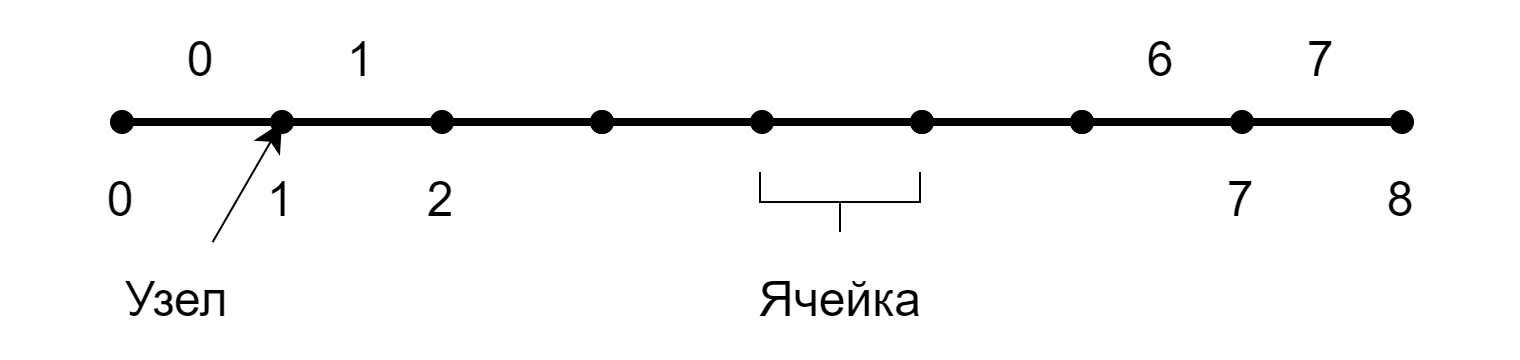
\includegraphics[width=\textwidth]{mesh1d}
	\caption{Одномерная сетка с номерами узлов снизу и номерами ячеек сверху\label{pic:mesh1d}}
\end{figure}

Первым делом выполняется разбиение расчетной области (в нашем случае -- отрезка) на маленькие отрезки. Это разбиение называется сеткой (см. рис. \ref{pic:mesh1d}). Точки разбиения называются узлами, а получающиеся отрезки -- ячейками. Вводя сетку с $N$ ячейками, мы имеем $N+1$ узлов и шаг сетки, то есть размер ячейки, равный $\Delta x = L/N$. Формально говоря, узлы имеют координаты $x_i = i\Delta x,~~i = 0, \dots, N$. Ячейка с номером $i$ представляет собой отрезок $[x_i, x_{i+1}]$.

Решением краевой задачи \eqref{eq:poisson_bvp_dir_1d} в классическом смысле является некоторая функция $u \in C^2(0,L) \cap C[0;1]$ и т.д. и т.п. В численном же решении мы будем искать набор значений в узлах:
\begin{equation}
	y_i \approx u(x_i),~~~i = 0, \dots, N.
\end{equation}

Поскольку значения в граничных узлах определяются граничными условиями, фактически задача сводится к поиску $y_1, ..., y_{N-1}$. 

Идея метода конечных разностей состоит в замене производных в уравнении на некоторые конечные разности. Так, например, можно использовать выражения
\begin{equation}\label{eq:differences_1}
	\begin{split}
		y_{x,i} = \frac{y_{i+1} - y_i}{\Delta x} = u'(x_i) + \mathcal{O}(\Delta x),\\
		y_{\overline{x},i} = \frac{y_i - y_{i-1}}{\Delta x} = u'(x_i) + \mathcal{O}(\Delta x),
	\end{split}
\end{equation}
называемые разностными производными вперед и назад. Оценки на погрешность аппроксимации справедливы для достаточно гладких функций.

Разностная аппроксимация второй производной имеет вид
\begin{equation}\label{eq:differences_2}
	\begin{split}
		y_{x\overline{x},i} \equiv y_{\overline{x}x,i} = \frac{y_{i+1} - 2y_i + y_{i-1}}{\Delta x^2} = u''(x_i) + \mathcal{O}(\Delta x^2).
	\end{split}
\end{equation}

Для определения значений $y_i$ составляется система линейных алгебраических уравнений. В каждом внутреннем узле исходное уравнение заменяется на разностную аппроксимацию:
\begin{equation}
	\begin{cases}
		-\frac{y_{2} - 2y_1 + a}{\Delta x^2} = f(x_1),\\
		-\frac{y_{3} - 2y_2 + y_1}{\Delta x^2} = f(x_2),\\
		\dots\\
		-\frac{y_{i+1} - 2y_i + y_{i-1}}{\Delta x^2} = f(x_i),
		\dots\\
		-\frac{b - 2y_{N-1} + y_{N-2}}{\Delta x^2} = f(x_{N-1})\\
	\end{cases}
\end{equation}

Если умножить все уравнения на $\Delta x ^2$, в матричном виде система принимает следующий вид:
\begin{equation}
	\begin{bmatrix}
		2  & -1 &   &       \\
		-1 &  2 & -1 \\
		   & -1 &  2 \\
		   &    &   & \ddots \\
		   &    &   &       &  & -1\\
		   &    &   &       & -1 & 2
		
	\end{bmatrix}
	\begin{bmatrix}
		y_1 \\ y_2 \\ y_3 \\ \vdots \\y_{N-2} \\ y_{N-1}
	\end{bmatrix}
	=
	\Delta x^2 
	\begin{bmatrix}
		f(x_1) + a/\Delta x^2 \\
		f(x_2)\\
		f(x_3)\\
		\vdots\\
		f(x_{N-2})\\
		f(x_{N-1}) + b/\Delta x^2 
	\end{bmatrix}
\end{equation}

Матрица системы является симметричной, знакоопределенной и разреженной (число ненулевых элементов порядка размера матрицы). Это типично для матриц, возникающих при дискретизации уравнений в частных производных. Часто 


\begin{thebibliography}{2}
	\bibitem{vas} Ю.В.Василевский, М.А.Ольшанский, Краткий курс по многосеточным методам и методам декомпозиции области \texttt{http://old.inm.ras.ru/library/Vassilevski/yuv-olsh-mnogoset-dekomp.pdf}
	\bibitem{gor} Горобец Андрей Владимирович,
	Параллельные методы решения задач\texttt{https://keldysh.ru/math-center/prj-reports/EPrj-04\_lectures.pdf}
\end{thebibliography}

\end{document}